\documentclass[]{final_report}
\usepackage{graphicx}
\usepackage{hyperref}
\usepackage[normalem]{ulem}
\usepackage{amsmath}
\usepackage{graphicx}
\usepackage{csvsimple}

%%%%%%%%%%%%%%%%%%%%%%
%%% Project details
%%%%%%%%%%%%%%%%%%%%%%
\def\studentname{Kamil Smuga}
\def\projecttitle{An approach for Continuous Capacity Planning in Cloud Environments with Uptime-based Pricing Model}
\def\supervisorname{Liam Murphy}
\def\moderatorname{Christina Thorpe}

\begin{document}

\maketitle
\tableofcontents\pdfbookmark[0]{Table of Contents}{toc}\newpage

%%%%%%%%%%%%%%%%%%%%%%
%%% ABSTRACT 
%%%%%%%%%%%%%%%%%%%%%%

\begin{abstract}

\textsl{New Infrastructure as a Service solutions are becoming available with a growing number of supported pricing models. More often than not, a hosted Cloud environment is used to design and build an infrastructure for a product. The recent availability of different pricing schemes based on resource utilization and uptime reveals new challenges in already unpredictable capacity planning process. There is a choice between ad-hoc provisioning and upfront payments with reduced hourly rates. Reserved instances charged upfront are categorized into three groups: light, medium and heavy. Which one is better for a given utilization model? When exactly does one pricing scheme becomes more cost effective? Determining which machine type is better for a given utilization model, or at which point the cost effectiveness of a pricing scheme changes, is vital for the companies subscribing to the IaaS. }

\end{abstract}
\newpage

%%%%%%%%%%%%%%%%%%%%%%
%%% INTRODUCTION 
%%%%%%%%%%%%%%%%%%%%%%

\chapter{Introduction}

\section{Objectives}

\section{Structure of the Document}

\newpage

%%%%%%%%%%%%%%%%%%%%%%
%%% BACKGROUND 
%%%%%%%%%%%%%%%%%%%%%%

\chapter{Background}

\section{The Problem Domain}

\section{Motivation}

\section{IaaS consumer point of view}

\section{IaaS provider uptime-based pricing schemes}

\section{Literature review}


%%%%%%%%%%%%%%%%%%%%%%
%%% OPTIMALITY 
%%% ALGORITHM 
%%%%%%%%%%%%%%%%%%%%%%

\chapter{Design and Implementation of Optimality Algorithm Based on Uptime and Pricing Scheme}

\section{Taxonomy}

\subsection{Upfront cost}

Investement in compute resources comes with upfront cost. In case of physical machine it is hardware or lease cost. For virtual resources, IaaS providers offer per hour discounts for upfront charged schemes. \par
Upfront cost is considered to be one time payment and will be represented by \textit{u}. 

\subsection{Cost per hour}

Cost per hour represents an aggregated cost of running a single machine divided by number of hours in a calendar year. Aggregate cost is relatively easy to calculate for virtualized environments. IaaS providers usually charge an X amount per hour. It might vary based on total uptime per month or pricing scheme. This number will be considered as partial cost per hour and defined as \textit{pcph}. \par
Cost of running of physical hardware is less straightforward to calculate as it includes: power consumption, operations, hardware replacements cost, data center related costs and many others that may vary based on individual cases. Although more troublesome to calculate, cost per hour per host for physical infrastructure is possible to calculate. \par
Cost per hour will be defined as \textit{cph}. Considering the fact that upfront cost is more substantial for light usage than 24/7, cost per hour will be defined as a function of hours/day usage defined as \textit{h} and calculated from equation:
\begin{equation}
cph(h) = \frac{u + \sum_{i=1}^{366} pcph \times h}{365 \times h}
\end{equation}
\section{Design}
\section{Implementation}

%%%%%%%%%%%%%%%%%%%%%%  
%%% ALGORITHM TESTING  
%%% ON GOOGLE DATASET 
%%%%%%%%%%%%%%%%%%%%%%

\chapter{Algorithm Testing on Google Cluster Usage Dataset}

\section{Input data assumptions} 

Based on data published for AWS~\cite{AWS:2014} 

\csvautotabular{out}

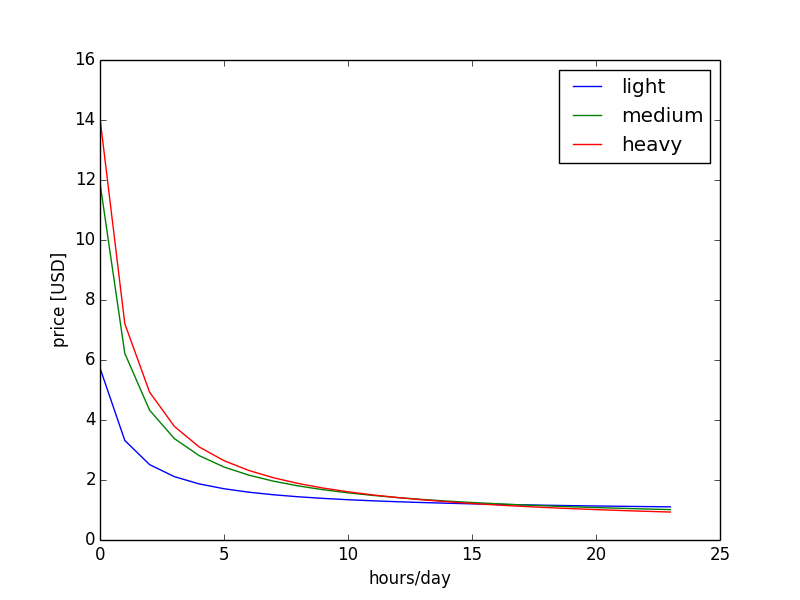
\includegraphics[width=\linewidth]{cph}
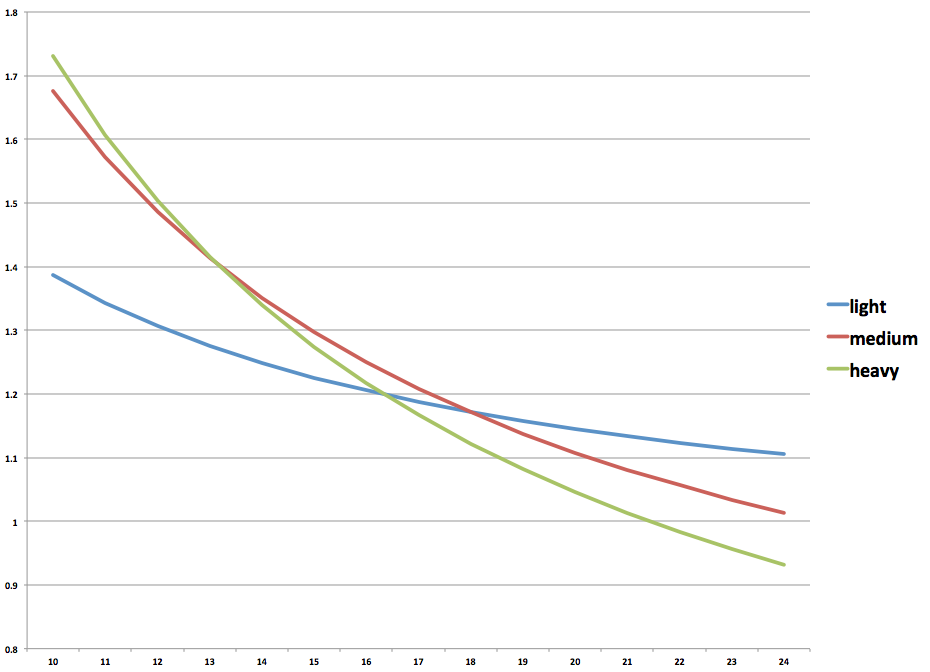
\includegraphics[width=\linewidth]{cph_zoom}

\section{Calculate cost per hour for each pricing scheme: light, medium and heavy}

\section{Graph price per hour on y and number of hours/day on x to find cut points}

\section{Calculate optimality factor based on distance from cut points}

%%%%%%%%%%%%%%%%%%%%%%
%%% CAPACITY PLANNING 
%%% STRATEGIES    
%%%%%%%%%%%%%%%%%%%%%%

\chapter{Capacity Planning Strategies}

\section{Peak-to-mean ratio based resource assignment}

\section{Only heavy instances}

%%%%%%%%%%%%%%%%%%%%%%
%%% CONCLUSION 
%%%%%%%%%%%%%%%%%%%%%%

\chapter{Conclusion and Further Work}

%%%%%%%%%%%%%%%%%%%%%%
%%% BIBLIOGRAPHY 
%%%%%%%%%%%%%%%%%%%%%%

\newpage
\begin{thebibliography}{99}
\bibitem{AWS:2014} http://forecastcloudy.net/2012/04/02/amazon-web-services-aws-ec2-pricing-data/ https://a0.awsstatic.com/pricing/1/deprecated/ec2/ri-light-linux.json https://a0.awsstatic.com/pricing/1/deprecated/ec2/ri-medium-linux.json https://a0.awsstatic.com/pricing/1/deprecated/ec2/ri-heavy-linux.json
\end{thebibliography}
\label{endpage}

\end{document}

\end{article}